\paragraph{Logo}
	Figura \ref{fig:logo_WIMC}
	\begin{figure}[h]
		\centering
		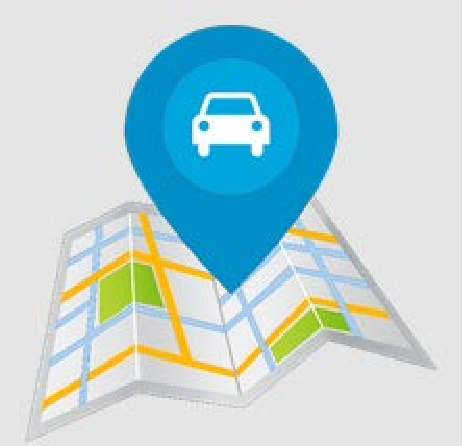
\includegraphics[scale=.6]{./analisisDeLaOferta/source/logo_WIMC}
		\caption{Logo WIMC}
		\label{fig:logo_WIMC}
	\end{figure}

\paragraph{Descripci�n}
Descripci�n
�Alguna vez estacionaste tu coche y se te olvid� d�nde lo hab�as dejado?
WIMC (Where's my car?) te permite guardar la posici�n de tu coche para que ya no lo vuelvas a perder.
Adem�s, permite obtener las indicaciones para llegar desde tu posici�n hasta el coche a trav�s de Google Maps y ver la informaci�n de los �ltimos lugares donde estacionaste.

Caracter�sticas:
\begin{itemize}
	\item Guardar la posici�n de tu coche.
	\item Obtener indicaciones sobre c�mo llegar.
	\item Informaci�n sobre �ltimos lugares, con fecha y tiempo de estacionamiento.
\end{itemize}

Pr�ximamente:
\begin{itemize}
	\item Guardar posici�n autom�ticamente cuando el dispositivo se desconecta del Bluetooth del coche.
	\item Sugerir posici�n autom�ticamente al detectar una pausa en el movimiento.
	\item Configuraciones de la aplicaci�n.
	\item Agregar comentario opcional al guardar la posici�n.
	\item Widget para guardar posici�n.
\end{itemize}

\paragraph{Precio}
	Gratis

\paragraph{Plataformas}
	\begin{itemize}
		\item Android
	\end{itemize}
	
\paragraph{Link}
	\begin{itemize}
		\item \url{https://play.google.com/store/apps/details?id=com.matiasguerra.wimc.app}
	\end{itemize}
		